% !TEX root = ../main.tex
%
\chapter{Introduction}
\label{intro}
The tremendous volume of information in the Internet started with Web 2.0 development. Web 2.0 established a paradigm shift where users actively participate and share data through applications such as blogs, social networks, or other web applications \citep{NEWMAN2016591}. %As time goes by, the information continues to grow at a feared rate, therefore data processing becomes challenging.
Since the amount of exchanged information grows everyday faster, data processing becomes even more challenging.

Figure \ref{fig:web} presents an example of interactions between users and applications, such as uploading or downloading music, commenting on a post, and receiving notifications, among many other possibilities.

\begin{figure}[!ht]
    \centering
    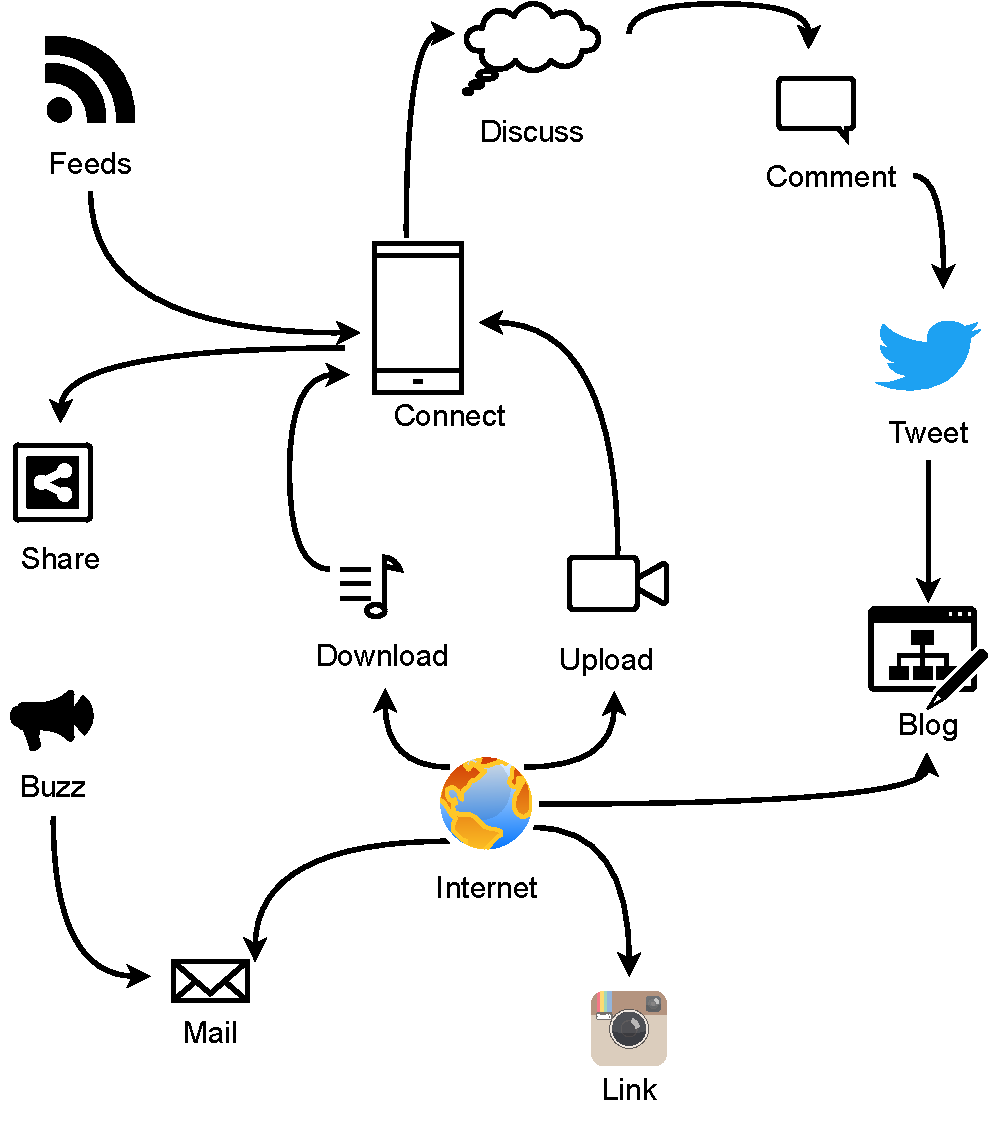
\includegraphics[width=0.4\textwidth]{figures/concepts/Web.pdf}
    \caption{Interactions on the Internet.}
    \label{fig:web}
\end{figure}

Data analysis for extracting information may be defiant. Such a task is even more complex if the analysis should take place in real-time. Under such a scenario, traditional processing systems based on the \textit{Batch processing} paradigm like \textit{MapReduce} \citep{DeanG08, CasadoY15} are not suitable for carrying out the analysis. Figure \ref{fig:batch-processing} shows a data pipeline using \textit{Batch processing}, where events are read to be processed periodically according to a time window, and, therefore, report are not generated online.

\begin{figure}[!ht]
    \centering
    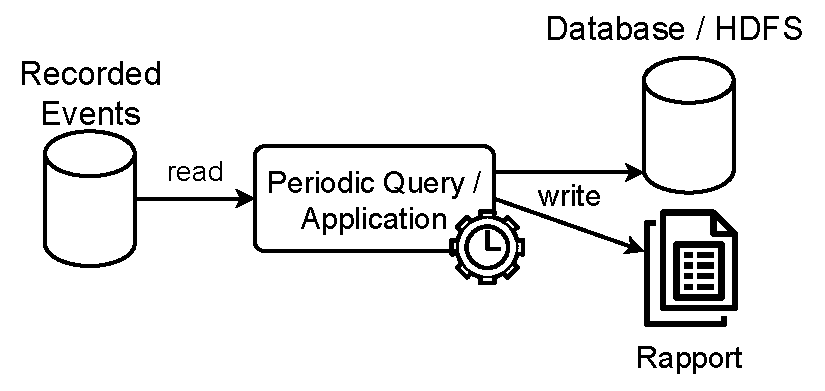
\includegraphics[width=0.7\textwidth]{figures/concepts/BatchProcessing.pdf}
    \caption{Batch processing concept.}
    \label{fig:batch-processing}
\end{figure}

Sustained on the need to process interactions in an online manner, different processing systems have been proposed in the literature. These systems are capable of dealing with unbounded sequences of events and deliver low-latency data. Nowadays, most users require quick and updated information online as a support for decision-making \citep{OzalRT11}.

A good example is social network analysis under post-disaster scenarios, where events are continuously generated, processing them as close to real-time as possible is necessary to obtain timely information to mitigate the disaster effects \citep{WladdimiroICTDM2016}. With such information, areas may be prioritized, resource distribution can be improved,  people searches may be more efficient, among others.

Another application is stock exchange prediction \cite{DingWPXL17}. In this case,  processing systems may analyze data and create mathematical models to predict the next day’s market behavior. 

In network security scenarios it is possible to monitor the network activity \citep{Zhao8230279}. As the data is processed in real-time, it may help to detect 'on the fly' malicious behaviors. A similar approach is followed on logs analysis. Online data processing makes it possible to detect bugs or errors, as well as to see if there is any intruder or system policy violation.

Stream Processing Systems (SPS) were specially designed to fulfill these needs \cite{Leibiusky0030281}. The goal of a SPS is to process unbounded continuous flows of events and to provide a scalable and efficient tool to process data close to real-time. Figure \ref{fig:stream-processing-concept} presents an example of a stream processing pipeline. Events are processed on the fly and aggregated results are stored in a database or presented on a dashboard.

\begin{figure}[!ht]
    \centering
    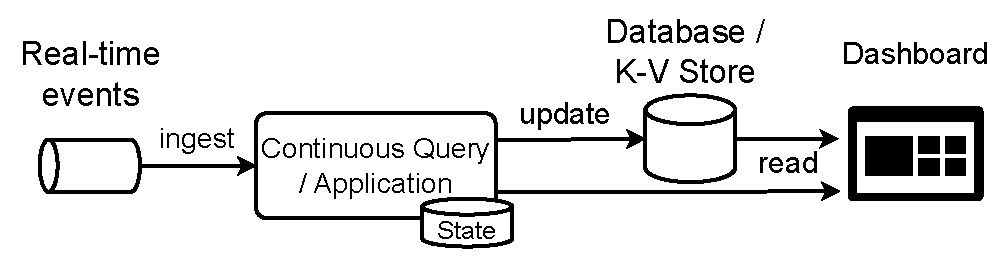
\includegraphics[width=0.95\textwidth]{figures/concepts/StreamProcessing-Concept.pdf}
    \caption{Stream processing concept.}
    \label{fig:stream-processing-concept}
\end{figure}

SPSs are based on directed acyclic graphs (DAG) whose vertices and unidirectional edges correspond to operators and event data flows respectively \cite{ChakravarthyJ09}. An external source continuously provides the data that the system consumes. Light programming tasks (like filters, counters, storage, etc.) are handled by operators that quickly and in pipeline-style process the data (events). In a processing infrastructure (e.g. clusters, clouds, etc.), resources (e.g., VMs) are allocated to execute the operators which are frequently replicated for performance reasons. Figure \ref{fig:sps-introduction} shows an example of a SPS application, whose pipeline is composed of one input data and four operators. In this example, each operator processes the events according to the pipeline flow, provided by the input data.

\begin{figure}[!ht]
    \centering
    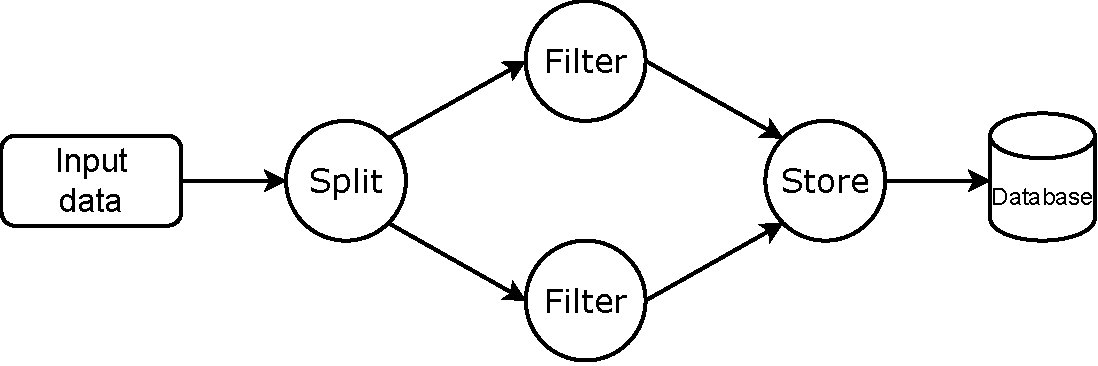
\includegraphics[width=0.95\textwidth]{figures/concepts/SPS-Introduction.pdf}
    \caption{Example of a SPS application.}
    \label{fig:sps-introduction}
\end{figure}

SPS frameworks, such as Storm \citep{Leibiusky0030281} or Flink \citep{CarboneKEMHT15}, are configured before their deployment, usually defining both the DAG and the number of operator replicas beforehand. There are works that adapt the number of replicas dynamically based on analysis of input fluctuation \citep{CardelliniPNR18, arkian2021model, KombiLLRB19}. However, replica reconfiguration usually requires stopping the application and restating it. For adapting the number of replicas, there exist basically two approaches. The reactive approach considers the state of the system, while the predictive analyses the history of the states.

Another critical feature of SPSs is the grouping strategy which is responsible for sharing the input load among operators' replicas. For instance, the round-robin policy is one of the most common approaches to implementing shuffle grouping.  However, the latter does not consider the input load of each replica, i.e., current queued events waiting to be processed.

The behaviour of data streams can be quite dynamic. Traffic behaviour may suddenly increase/decrease, and event distributions may be unbalanced, among others.  Such a dynamics may create struggle operators, increasing end-to-end latency and message loss. To solve this problem it is necessary to dynamically adapt the processing logic of the SPS, thereby increasing or decreasing the number of replicas of an operator, so a good adaptation decision may minimize the aforementioned problem: the latency and message loss can be reduced reaching higher accuracy for the data analysed.

For this reason, one solution is to propose an adaptive SPS, which characterize system utilization requirements and automatically increase/decrease the number of replicas of critical operators to keep latency restrictions and reduce event loss.

\section{Contributions}
\label{contributions}

%% 1. INTRODUCTION
This thesis proposes two adaptive SPSs (\rSPS{} and \pSPS{}) based on Storm \citep{toshniwal2014storm}. Its aim is to adapt the number of replicas of the operators according to the sparks in the data stream.
%% 2. MAPE Approach
Both adaptive SPS use the MAPE model \citep{ibm2005architectural}, which consists of a control loop composed of four modules: Monitoring, Analysis, Planning, and Execution.

%% 3. RA-SPS + PA-SPS
\rSPS{} and \pSPS{} exploit a reactive and predictive approach respectively. \rSPS{} bases its decision on the state of an operator at runtime, according to the analysis of traffic peaks in short periods of time.  \pSPS{} bases its decision on the behaviour of the input data and the number of operator active replicas required for processing the input data, finding patterns in the traffic to anticipate possible overloads, or underloads in the SPS.

%% 4. POOL
In order to cope with stream fluctuation both SPS, use a pool of operator replica, created beforehand. These replicas may be either active or inactive. Active replicas are deployed by the Storm scheduler. On the other hand, inactive replicas are idle, so they do not consume CPU resources but can be allocated as needed. Consequently, \textit{a pool of replicas} can be dynamically activated (resp., deactivated) when the system detects the need for increasing (resp., decreasing) the number of active replicas of an operator. Note that under this model, the stream processing systems can adapt without stopping the SPS.

%% 5. GROUPING
Another feature introduced in the proposed SPSs is the load-aware grouping that partitions the stream among replicas based on their respective current load.

%% 6. RA-SPS
\rSPS{} dynamically modify the number of replicas per operator based on a multi-metric. The multi-metric is composed of system statistics such as the queue size, the average execution time of an event, and the utilisation rate of an operator. It determines the state of the operators during a time interval, and depending on the state of the operator and conditions of the SPS, it is decided whether or not to modify the number of replicas.

%% 7. PA-SPS
\pSPS{} dynamically allocates the number of replicas per operator necessary to process the input stream, defining the events that each operator $O$ should process within a time interval. In order to predict the input stream and analyse the system's potential future behaviour, a predictive model is proposed, integrated to \pSPS{}. By considering both (1) the events sent to an $O$ by its direct operator predecessors as well as those from earlier time intervals that $O$ could not process at the time,  therefore, kept in a queue and (2) event execution time, the ideal number of $O$'s replicas for processing these events at each interval is deduced. As a result, the number of $O$'s replicas changes over time, depending on the input rate.

%% 8. EXPERIMENTS
This proposal is evaluated over the infrastructure of a well-known cloud provider, the Google Cloud Platform (GCP).  Performance was an exhaustive evaluation in terms of classical metrics such as end-to-end latency, resource utilization, the number of processed events, and the error of our estimations. This work presents, analyses, and discusses the results also comparing them with state of the art solutions. 

\section{Publications}
\label{publications}

Two articles in international conferences, two articles in French conferences, and one journal article submission under review. Chapter \ref{solution} presents the contributions of each article.

\subsection{International Conferences}
\begin{itemize}
	\item \cite{WladdimiroNCA} Daniel Wladdimiro, Luciana Arantes, Pierre Sens and Nicolas Hidalgo. "A Multi-Metric Adaptive Stream Processing System." In: \textit{NCA}. IEEE, 2021.
	\item \cite{WladdimiroSBAC} Daniel Wladdimiro, Luciana Arantes, Pierre Sens and Nicolas Hidalgo. "A predictive approach for dynamic replication of operators in distributed stream processing systems" In: \textit{SBAC}. IEEE, 2022.
\end{itemize}

\subsection{Journal}
\begin{itemize}
	\item \cite{WladdimiroJPDC} Daniel Wladdimiro, Luciana Arantes, Pierre Sens and Nicolas Hidalgo. "PA-SPS: A Predictive Adaptive Approach for an Elastic Stream Processing System" In: \textit{JPDC}. 2023. \textit{\textbf{[Under Review]}}
\end{itemize}

\subsection{National Conferences}
\begin{itemize}
	\item \cite{WladdimiroComPAS2022} Daniel Wladdimiro, Luciana Arantes, Pierre Sens and Nicolas Hidalgo. "A predictive model for Stream Processing System that dynamically calibrates the number of operator replicas." In: \textit{ComPAS}. Amiens, France, 2022.
	\item \cite{WladdimiroComPAS2023} Daniel Wladdimiro, Luciana Arantes, Pierre Sens and Nicolas Hidalgo. "PRESPS: a PREdictive model to determine the number of replicas of the operators in Stream Processing Systems" In: \textit{ComPAS}. Annecy, France, 2023.
\end{itemize}

\section{Organization}

The remaining of this theses is organised as follows:

%Chapter \ref{intro} was an introduction to the problem of real-time data processing, as well as an explanation of the adaptability problem in a SPS.

Chapter \ref{background} gives the necessary concepts for the understanding of SPSs, the architecture of the SPS frameworks, and our contribution.

Chapter \ref{related-work} presents related work about adaptive SPS. Existing solutions use a manual approach, which depends on a user for modifying the SPS, or a automatic approach, where the SPS is in charge of the adaptation.

Chapter \ref{solution} presents the proposed SPSs(\rSPS{} and \pSPS{}) as well as the pool of replicas and \textit{Load-Aware} grouping approach.

Chapter \ref{experimentation} presents evaluation results related to \rSPS{} and \pSPS{} experiments conducted on GCP.

Finally, Chapter \ref{conclusion} presents the conclusion and some future work.